\documentclass{standalone}
\usepackage{pgfplots}
\pgfplotsset{compat=1.18}

\begin{document}
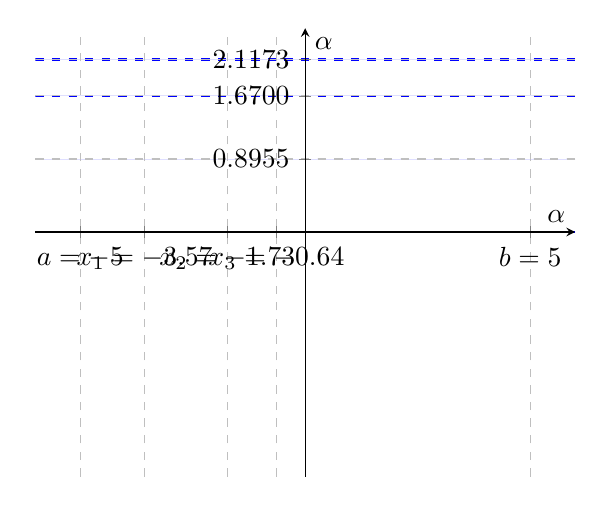
\begin{tikzpicture}
    \begin{axis}[
        axis lines=middle,
        axis on top,
        xmin=-6, xmax=6,
        ymin=-3, ymax=2.5,
        xtick={-5,-3.57,-1.73,-0.64,5},
        xticklabels={$a=-5$, $x_1=-3.57$, $x_2=-1.73$, $x_3=-0.64$, $b=5$},
        ytick={0,0.8955,1.6700,2.1173},
        yticklabels={$0$, $0.8955$, $1.6700$, $2.1173$},
        xlabel=$\alpha$,
        ylabel=$\alpha$,
        grid=major,
        grid style=dashed,
        domain=-6:6,
        samples=100,
        no markers,
        every axis plot post/.append style={
            thick,
            color=blue,
            dashed
        },
        every axis plot/.append style={
            thick,
            color=red,
            dashed
        }
    ]
        \addplot [fill=gray!20] coordinates {
            (-6, 0) (6, 0)
        };
        \addplot [fill=gray!20] coordinates {
            (-6, 0.8955) (6, 0.8955)
        };
        \addplot [fill=gray!20] coordinates {
            (-6, 1.6700) (6, 1.6700)
        };
        \addplot [fill=gray!20] coordinates {
            (-6, 2.1173) (6, 2.1173)
        };
    \end{axis}
\end{tikzpicture}
\end{document}